%TCIDATA{LaTeXparent=0,0,relatorio.tex}
\ifx\compilewholereport\undefined  
	\documentclass[11pt,a4paper,oneside]{book}
	
	% Escolher um dos seguintes formatos:
	\usepackage{ft2unb} % segue padrão de fontes do Latex
	
	% Pacotes
	\usepackage{graphicx}
	\usepackage{amsfonts}
	\usepackage{amsmath}
	\usepackage{amssymb}
	\usepackage[thmmarks,amsmath]{ntheorem}
	\usepackage{boxedminipage}
	\usepackage{theorem}
	\usepackage{fancybox}
	\usepackage{fancyhdr}
	\usepackage{url}
	\usepackage{afterpage}
	\usepackage{xcolor}
	\usepackage{rotating}
	\usepackage{makeidx}
	\usepackage{indentfirst}
	\usepackage{subcaption}
	\usepackage{todonotes}
	\usepackage{listings}
	\presetkeys{todonotes}{inline}{} 
	
	\begin{document}
	\frontmatter
	\tableofcontents
	\mainmatter 
	
	%%%%%%%%%%%%%%%%%%%%%%%%%%%%
	%%%%%%%% Apagar coisas acima
	%%%%%%%%%%%%%%%%%%%%%%%%%%%%
	\newcommand\qt[1]{\lq\lq{}#1\rq\rq{}}
	\newcommand\qti[1]{\lq\lq{}\textit{#1}\rq\rq{}}
\fi
                      
\chapter{Resultados}\label{CapExperimentos}

% Resumo opcional. Comentar se não usar.
\resumodocapitulo{Este capítulo tem como objetivo apresentar um resumo dos resultados alcançados pelos vários experimentos realizados, uma vez que os resultados específicos estão contidos nos capítulos dos respectivos experimentos.}
\vspace{0.8cm}

Os experimentos realizados neste trabalhos serviram para construir um conhecimento profundo em torno do desenvolvimento de aplicações reconfiguráveis baseadas em FPGAs.
Entende-se que as partes mais importantes deste conhecimento, além da capacidade de resolução de problemas relacionados, é o entendimento do fluxo de desenvolvimento necessário.
Este fluxo, resumido na figura \ref{fig:res:prfileflow}, não é descrito claramente na literatura, tornando esta tecnologia complicada de se estudar e utilizar.
O que buscou-se fazer com os experimentos foi determinar uma linha de pensamento sólida e lógica, que ajudasse a determinar este fluxo mais facilmente.

\begin{figure}[htp]
\centering
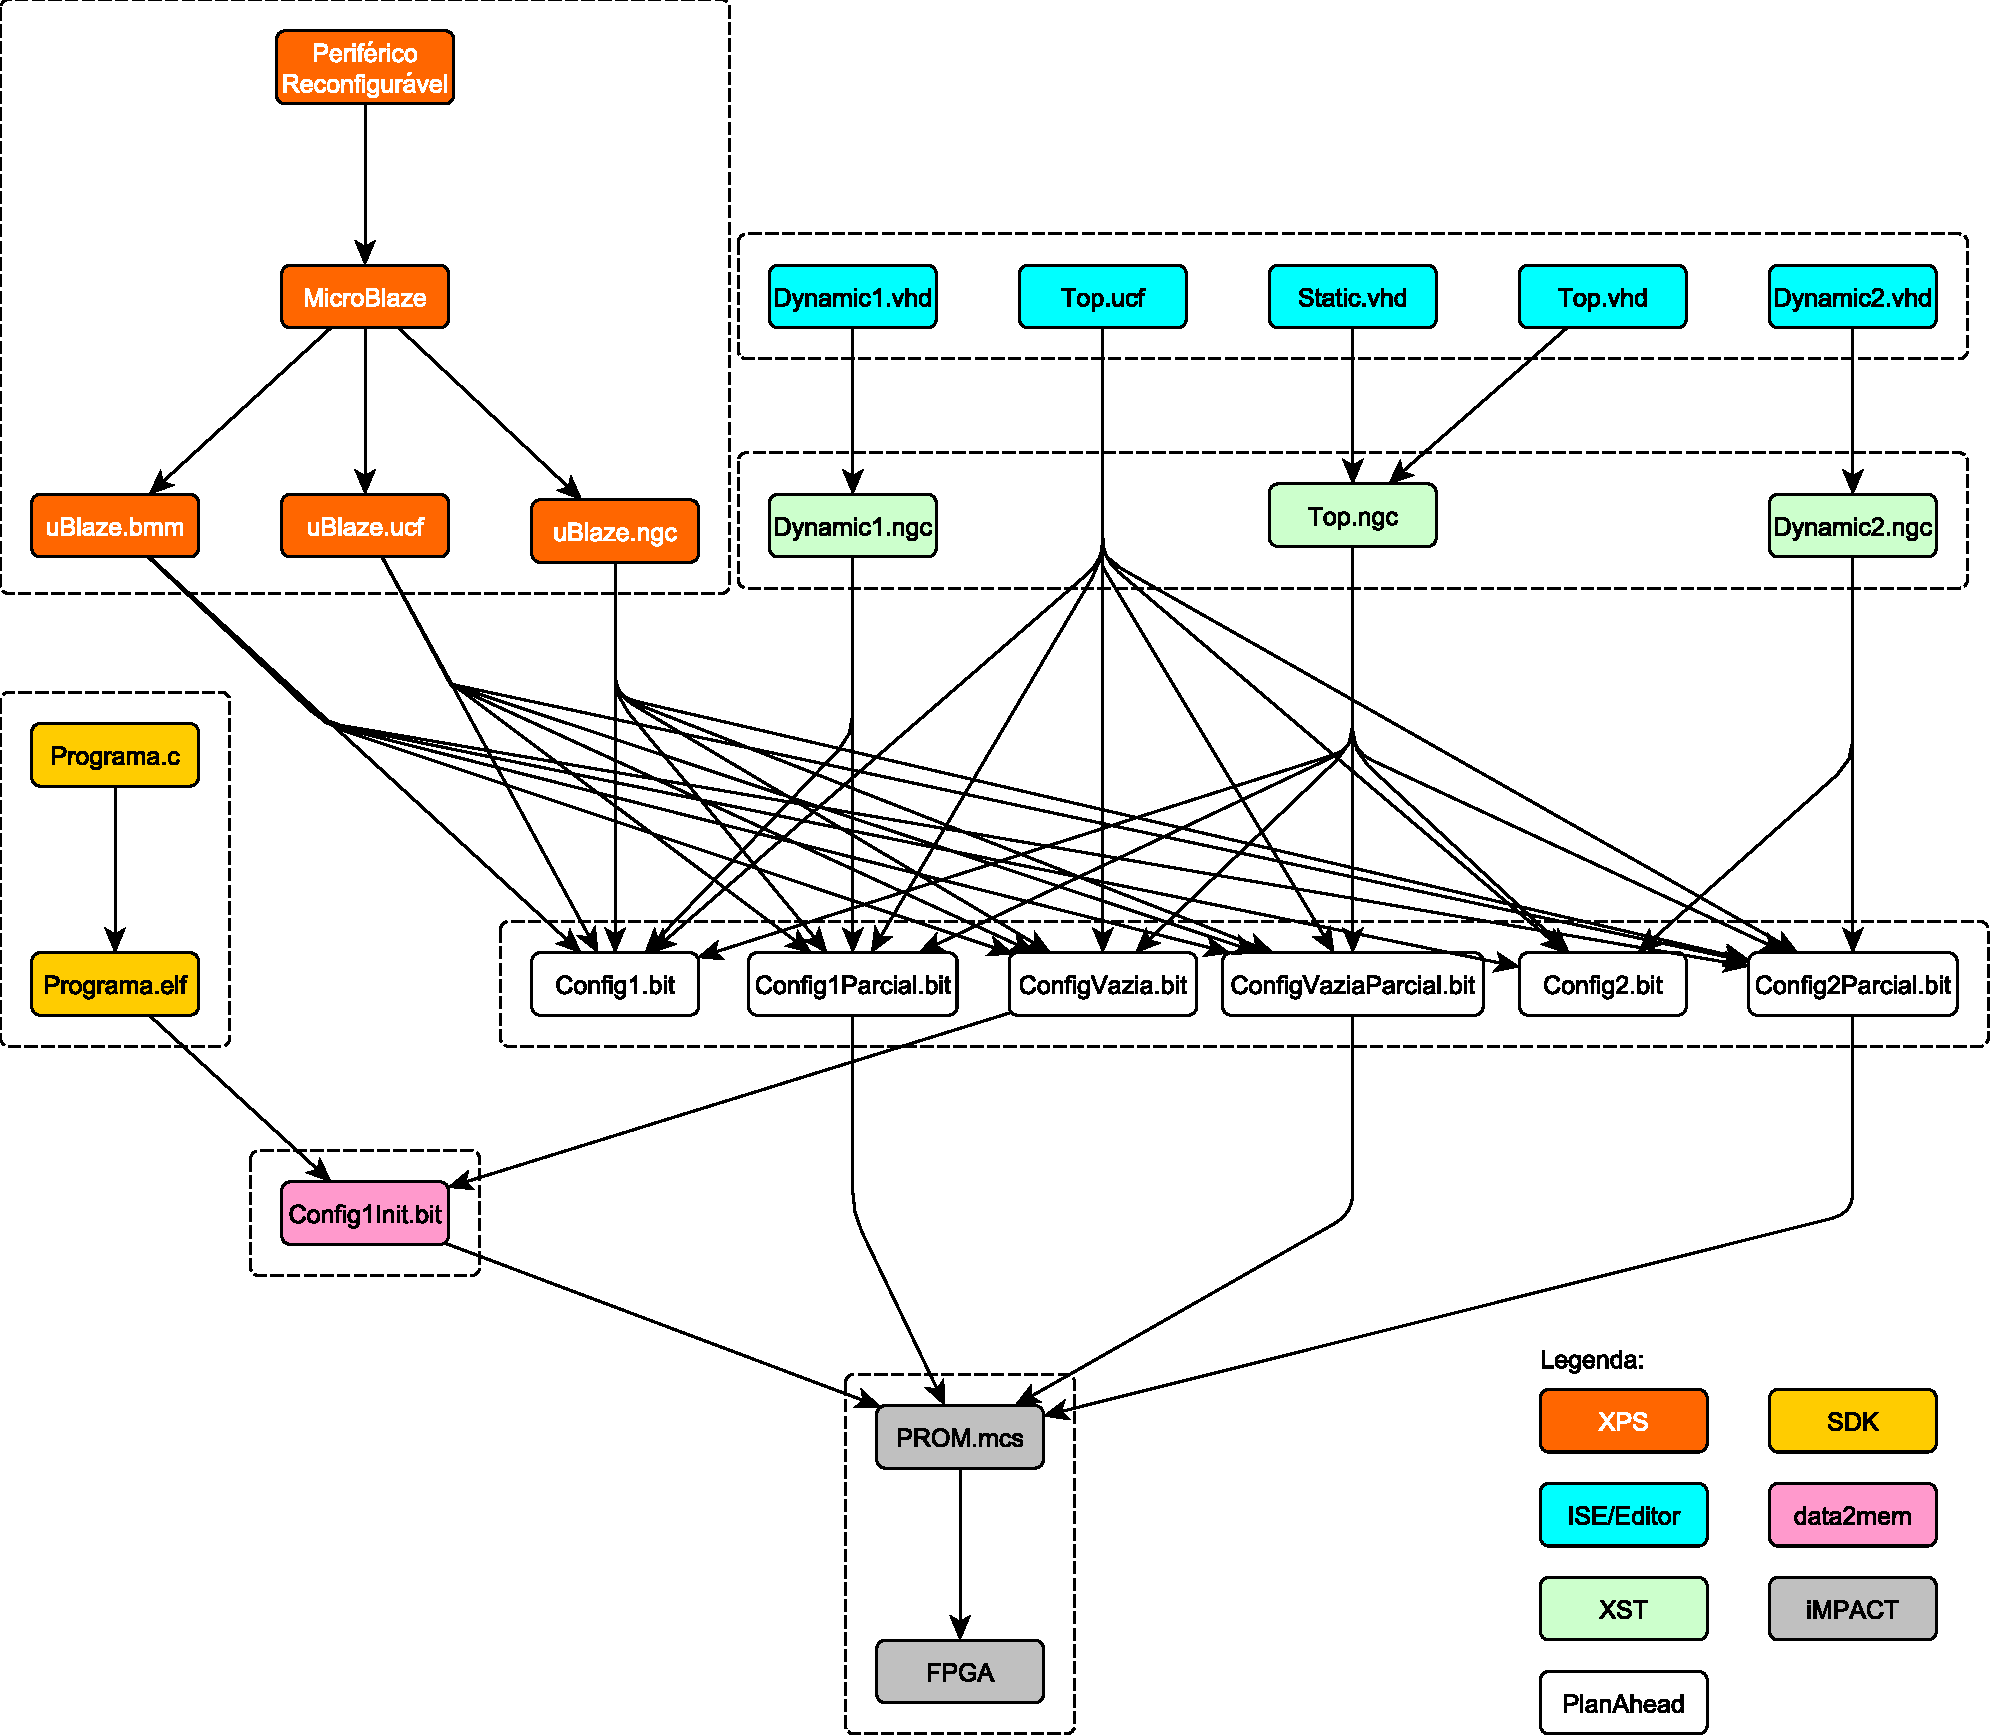
\includegraphics[width=\textwidth]{fig/resultados/prfileflow.pdf}
\caption{Fluxo de projeto para aplicações reconfiguráveis usando as ferramentas da Xilinx. Cada bloco representa um arquivo gerado com o auxílio de alguma ferramentas. As arestas indicam que tal arquivo foi utilizado para gerar o seguinte. Arquivos gerados pelas mesmas ferramentas estão agrupados com uma linha contínuo, no caso de um arquivo de construção obrigatória, ou com uma linha tracejada, no caso de arquivos cuja construção depende dos requisitos do projeto. Estão indicados ainda os tempos, incluindo os tempos das interações necessárias com o usuário, estimados para a construção de cada arquivo. Note que este fluxo é apenas o indicado para a maioria dos projetos, mas que existem projetos que seguem fluxos diferentes, seja por opção ou necessidade.}
\label{fig:res:prfileflow}
\end{figure}

Devido ao caráter de estudo de um tecnologia, não se faz necessária a inclusão de relatórios de utilização ou desempenho.
Estes elementos podem ser estudados mais a fundo de forma separada.
Sua inclusão neste trabalho poderia acarretar na perda do foco principal, quiça autorreconfiguração.

É interessante notar que um dos experimentos, especificamente o quarto, teve de ser reavaliado, tendo sido considerado mal sucedido.
O motivo para tal foi o encontro de diversos problemas graves que desaceleraram o desenvolvimento, comprometendo a realização deste trabalho.
Estes problemas foram causados em parte pela má integração entre as diversas ferramentas da Xilinx, mas em maior parte por problemas relacionados a memória DDR3 e seus requisitos de temporização.
Apesar disso, conseguiu-se perceber este impasse a tempo e reformular este experimento de tal forma que ele fosse alcançavel.

Através da realização dos experimentos de 1 a 4, juntou-se o conhecimento necessário que culminou na realização do experimento 5.
Este por sua vez, serviu para clarificar alguns detalhes referentes a integração de projetos do XPS e do PlanAhead, abrindo um leque de possibilidades de continuação deste trabalho.

\section{Análise de Tempo}
O fator mais explicitamente influenciador dos resultados deste projeto foi o tempo, especialmente quando aliado ao caráter experimental deste projeto.
Pode-se observar da figura \ref{fig:res:prfileflow} que cada ferramenta possui um tempo máximo e mínimo necessários para seu uso.
Estes tempos foram estimados com base nos tempos gastos nos experimentos, considerando-se que nenhum erro grave tenha acontecido.

A figura \ref{fig:res:prtimeflow} possui uma representação alternativa, que mostra a construção do projeto como um \textit{pipeline}.
As informações acima deste grafo direcionado representam os tempos, máximo e mínimo, gastos em cada etapa e as informações abaixo mostram o tempo gasto acumulado, máximo e mínimo, desde o início do projeto.
Note que, mesmo desconsiderando-se os tempos de desenvolvimento de periféricos, programas embarcados e comportamento do \textit{hardware}, leva-se no mínimo 1 hora e 47 minutos.
Considerando-se ainda que a maior parte dos erros é apresentada na etapa final da ferramenta PlanAhead, pode-se observar que gastou-se pelo menos 1 hora e 30 minutos por tentativa de implementação.

\begin{figure}[htp]
\centering
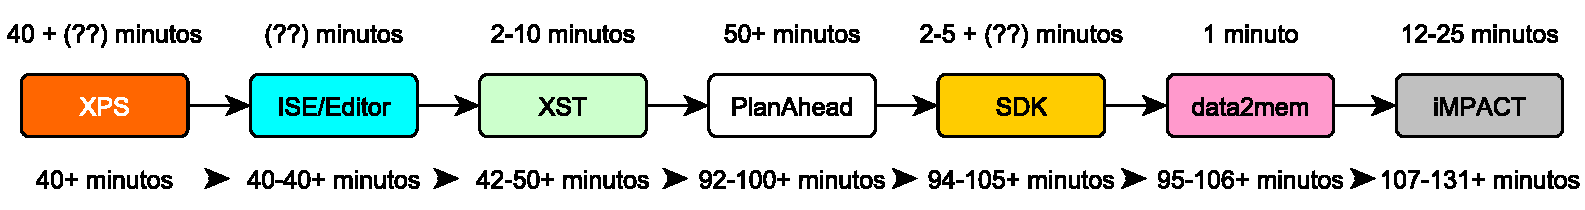
\includegraphics[width=\textwidth]{fig/resultados/prtimeflow.pdf}
\caption{Representação do fluxo de projeto através de um \textit{pipeline}. As informações acima dele indicam o tempo mínimo e máximo gasto em cada etapa, sendo que as etapas que possuem alguma fase de desenvolvimento apresentam um \lq\lq{}(??)\rq\rq{} para indicar que não tem como estimar o tempo gasto. As informações abaixo indicam o tempo mínimo e máximo gasto acumulado desde o início do projeto. A presença do sinal \lq\lq{}+\rq\rq{} indica que o valor apresentado é apenas uma estimativa empírica do valor máximo, podendo este ser ainda maior.}
\label{fig:res:prtimeflow}
\end{figure}

\ifx\compilewholereport\undefined
	\bibliographystyle{plain}
	\newsavebox\mytempbib\savebox\mytempbib{\parbox{\textwidth}{\bibliography{bibliografia}}}

	\listoftodos
	\end{document}
\fi